\documentclass{templateNote}
\usepackage{tcolorbox}
\usepackage{hyperref}
\usepackage{amsmath}
\usepackage{amssymb}
\usepackage{soul}
\usepackage{circuitikz}
\usepackage{float}
\usepackage[inline]{enumitem}
\usepackage{multicol}
\usepackage{colortbl}
\usepackage{tikz}
\usepackage{xcolor}
\usepackage[table]{xcolor}



\begin{document}
\imagenlogoU{img/logoNGMFormal_sinF.png}
\linklogoU{https://github.com/NicoGomezM} 
% \imagenlogoD{img/logo-ubb-txt-face.png} 
\titulo{Unidad 1}
\asignatura{Arquitectura de Computadores}
\autor{
    \indent
    Nicolás {Gómez Morgado}
}


\portada
\margenes 
\tableofcontents
\newpage

\section{Conceptos a tener en cuenta}
\begin{itemize}
    \item \textbf{Informática:} Ciencia de la computación. Conjunto de conocimientos científicos y técnicos que hacen posible el tratamiento automático de la información por medio de computadoras.
    \item \textbf{Computadora:} Maquina electronica, analógica o digital, que recibe, procesa y almacena información.
    \item \textbf{Computación:} Se refiere a un proceso matemático que genera una forma de información. 
    \item \textbf{Voltaje:} Potencial de fuerza que permite transferencia de corrientes eléctricas.
    \item \textbf{Programación:} Indicar a la computadora que hacer.
    \item \textbf{Programa:} Conjunto de instrucciones que le indican a la computadora que hacer con el fin de resolver un problema.
    \item \textbf{Arquitectura de computadores:} Todo dispositivo que nos permita manejar información, es decir, que pueda realizar operaciones matemáticas.
    \item \textbf{Mapas de Karnaugh:} Son una herramienta que nos permite simplificar funciones booleanas. Se utilizan para simplificar funciones booleanas de hasta 4 variables. Si se quiere comprobar que 2 circuitos son iguales sin las expresiones booleanas, se debe generar la tabla de verdad de ambos circuitos y compararlos.
    \item \textbf{Bit:} Unidad básica de información, puede ser 0 o 1.
    \item \textbf{Runtime:} Tiempo de atención a eventos/instrucciones en nanosegundos.
    \item \textbf{Buses:} Los que se encargan de la comunicación haciendo todo el recorrido. 
\end{itemize}
\newpage

\section{Principios Técnicos}
\noindent Von Neumann \textbf{no definió} la arquitectura de computadores, sino que agregó un concepto básico que transformó la computación: \underline{la memoria y la CPU se encuentran en el mismo lugar}, lo que permite que la CPU pueda acceder a la memoria de manera directa. 
\\\\
Turing demostró que se pueden crear máquinas decodificadoras. Esto dio paso a la computación de hoy en día y a la transferencia de datos a través de la red.
\\\\
Los \textbf{bits} son los que determinan la velocidad/calidad de un computador, mientras que los \textbf{bytes} son los que determinan la capacidad de almacenamiento de un computador.

\begin{tcolorbox}[colback=blue!5!white,colframe=blue!75!black,title=Ley de Moore]
En 1965, Gordon Moore gráfico los datos sobre el crecimiento en el rendimiento de la CPU de las computadoras, con lo cual predijo que cada nuevo chip doblaba la capacidad de su predecesor de hace 2 años (aumento exponencial).
\end{tcolorbox}

\noindent El procesador trabaja todo en lo que se llama registro. Este es como un vector de bits y su tamaño (32 o 64) determinará cuántas operaciones complejas puede realizar.

\subsection{Bytes}
\begin{table*} [H]
    \centering
        \renewcommand{\arraystretch}{1.5} % Aumenta la altura de las filas
        \begin{tabular}{|c|c|c|}
            \hline
            \textbf{Nombre} & \textbf{Nº Bytes} & \textbf{Equivalente}\\
            \hline
            Bit & Unidad básica &\\
            \hline
            Byte & $\displaystyle 2^0$ & 8 bit = 1 carácter \\
            \hline
            Kilobyte & $\displaystyle 2^{10}$ & 1024 B \\
            \hline
            Megabyte & $\displaystyle 2^{20}$ & 1024 kB \\
            \hline
            Gigabyte & $\displaystyle 2^{30}$ & 1024 mB \\
            \hline
            Terabyte & $\displaystyle 2^{40}$ & 1024 Gb \\
            \hline
            Petabyte & $\displaystyle 2^{50}$ & 1024 Tb \\
            \hline
        \end{tabular}
    \label{tab:componentes}
\end{table*}

\noindent \textit{\textbf{¿Qué es un byte y por qué tiene 8 bits?}} \\
Un byte es una \textbf{unidad básica de información} que consiste en 8 bits. La razón por la cual un byte tiene 8 bits se debe a que 
\textbf{256 es el número de combinaciones estandarizadas posibles} con 8 bits, lo que permite representar el \textbf{total de caracteres} en 
un conjunto de caracteres. El rango de caracteres representables va desde 0 hasta 255, lo que abarca la mayoría de los caracteres 
utilizados en diferentes sistemas de escritura. En caso de que se necesite representar números positivos y negativos la mitad de 
las combinaciones se utilizan para los números negativos y la otra mitad para los números positivos (127 y 127 implicando un 0 y un -0).
\\\\
\noindent \textit{\textbf{¿El programa que voy a utilizar cabe completamente en la RAM?}} \\
Típicamente no. El proceso que voy a describir se conoce como segmentación de código. En términos estrictos, se le llama paginación. 
El uso de la paginación se suele dar cuando tratamos con programas de gran tamaño.
La paginación implica que el sistema acceda al \textbf{disco duro} para buscar las instrucciones que se ejecutarán en la \textbf{RAM}. Esto se realiza 
en trozos, siendo la cantidad de trozos igual a la cantidad en que se dividió el programa. La máquina no toma decisiones al respecto, 
simplemente asigna espacios iguales en la RAM para los programas en ejecución, independientemente de si uno ocupa más o menos memoria. 
Es decir, no se borra, simplemente se \textbf{sobrescribe}.
\\\\
\noindent \textit{\textbf{¿Cuál es más eficiente, tener la máquina ejecutando un solo programa o varios programas?}}\\
En términos de eficiencia, es preferible tener menos programas en ejecución, ya que \textbf{cuantos más programas se ejecuten simultáneamente, más se divide la RAM}, 
asignando espacios iguales de memoria sin importar si un programa está siendo utilizado activamente o no. Se recomienda utilizar solo lo necesario para evitar
esta fragmentación.
\\\\
\noindent \textit{\textbf{¿Cuántos bytes ocupa un número entero en C?}}\\
En C, un número entero (int) generalmente ocupa 4 bytes (anteriormente ocupaba 2 bytes). Esto permite un total de $2^{32}$ combinaciones de números, con la mitad 
menos 1 para los valores positivos y el mismo valor para los valores negativos, con un cero tanto positivo como negativo.

\begin{tcolorbox}[colback=green!5!white,colframe=green!75!black,title=Ejercicio]
    \textbf{Ejercicio 1:} \\
    ¿Cuántos bit hay en 4 Tb? \\
    \begin{center}
        \textbf{Solución:} \\
        1 Tb = $2^{40}$ bits = 1024 Gb\\
        4 Tb = 4$\times2^{40}$ = $2^{2}\times2^{40}$ = $2^{42}$ bits.

    \end{center}
\end{tcolorbox}

\noindent \textit{\textbf{¿Qué consume más en un disco duro?}}\\
Lo que más consumiría serían los \textbf{byte de dirección} puesto que al pasar los $256$ datos posibles se usa 1 byte más para direcciones aumentando las posibilidades. 

\begin{tcolorbox}[colback=green!5!white,colframe=green!75!black,title=Ejercicio]
    \textbf{Ejercicio 2:} \\
    ¿Cuantos bytes de dirección hay en 8 Tb de datos? \\
    \begin{center}
        \textbf{Solución:} \\
        8 Tb = 8$\times2^{40}$ = $2^{3}\times2^{40}$ = $2^{43}$ byte.\\
        Para: \\
        $2^{8}\rightarrow 1 $\space$byte \times$ dato \\
        $2^{16}\rightarrow 2 $\space$byte \times$ dato \\
        $\vdots$ \\
        $2^{40}\rightarrow 5 $\space$byte \times$ dato \\
        $2^{48}\rightarrow 6 $\space$byte \times$ dato \\
    \end{center}
    \textit{Para este ejemplo 1 byte de datos esta acompañado de 6 bytes de dirección}.
\end{tcolorbox}

\noindent \textbf{\textit{Si un disco duro o respaldo indica que tiene 128 GB de almacenamiento, ¿se refiere esa cifra a bytes de datos y direcciones?}} \\
Normalmente, cuando se menciona una capacidad de almacenamiento, no se incluyen explícitamente las capacidades de direccionamiento. Por lo tanto, se puede concluir 
que la cifra de 128 GB se refiere únicamente a la capacidad de almacenamiento de datos, sin tener en cuenta la capacidad de direccionamiento.


\newpage

\section{Arquitectura de una computadora} 
\noindent Arquitectura de una computadora según Von Neumann:
\begin{figure}[H]
    \centering
    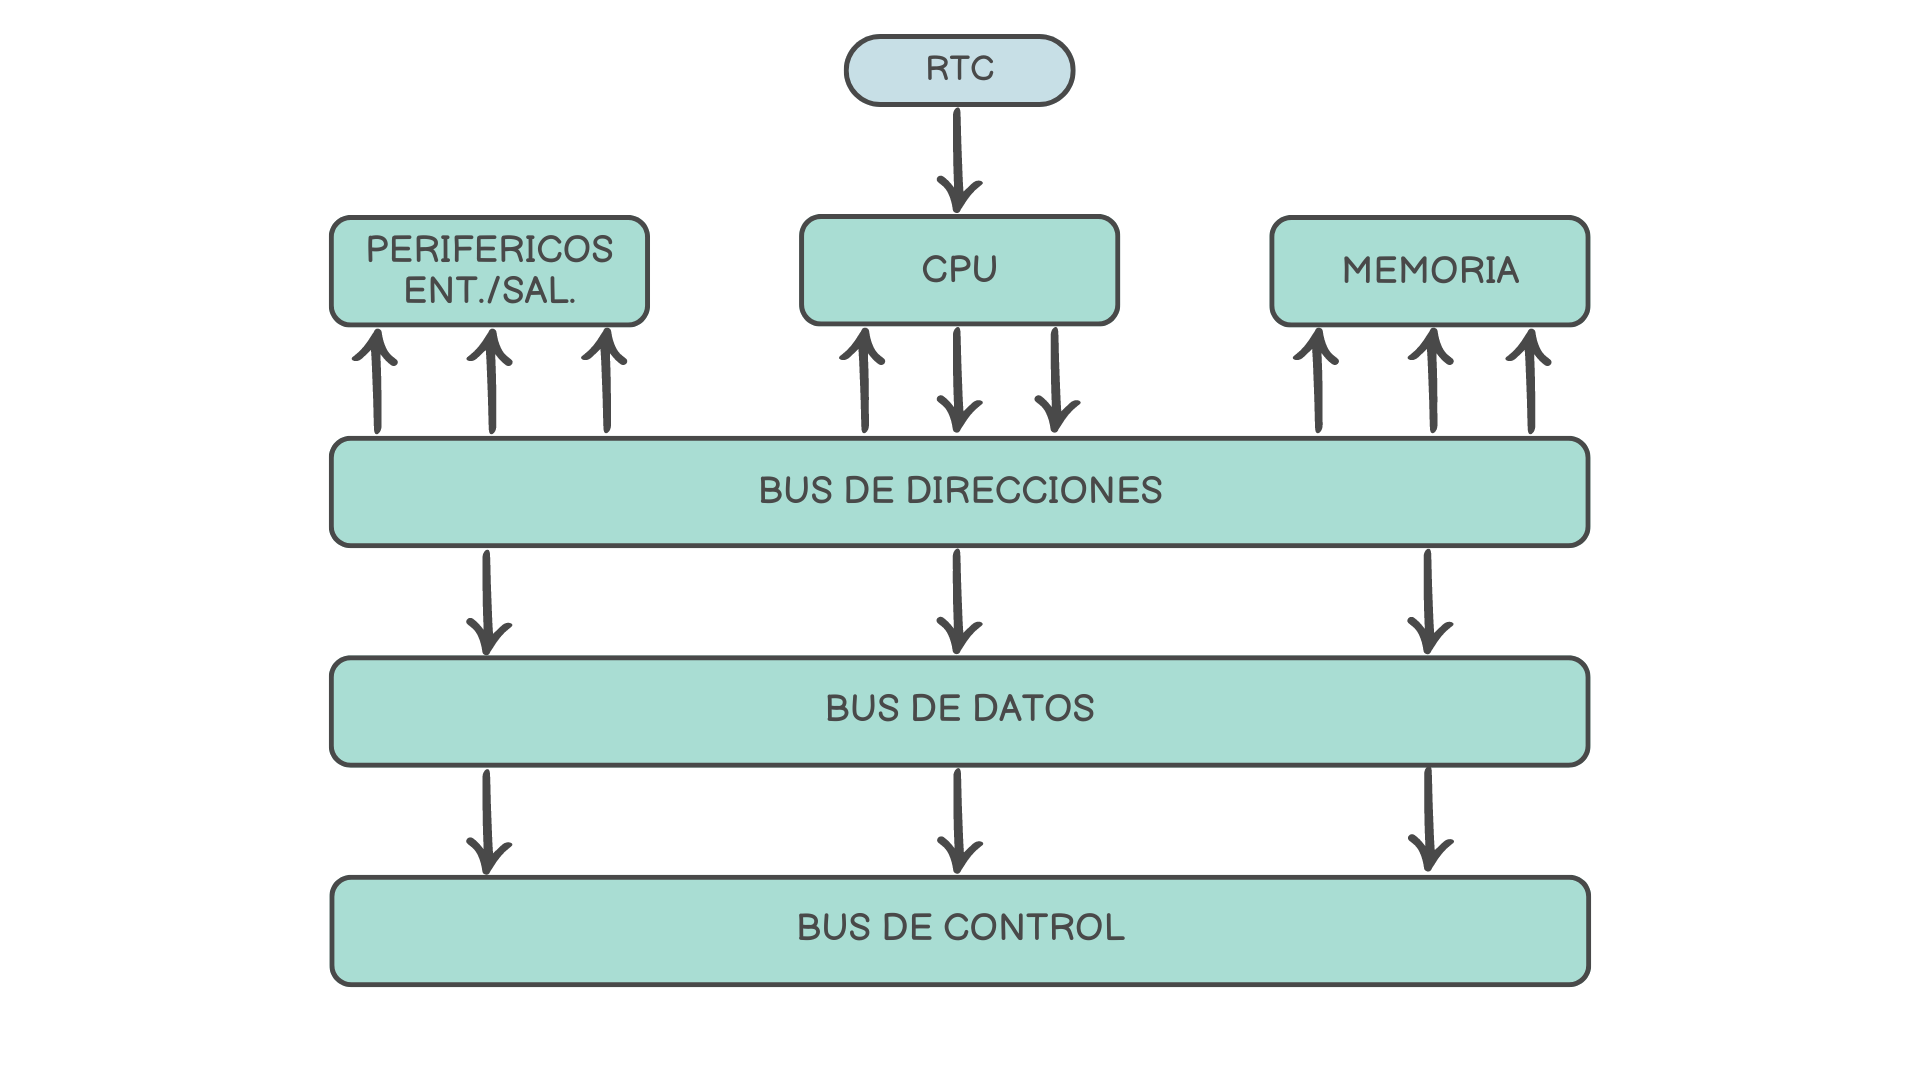
\includegraphics[height=7cm]{img/compubasica.png}
\end{figure}

\subsection{Conexiones y buses}
\begin{itemize}
    \item \textbf{Bus de direcciones:} Permite que el CPU y los periféricos accedan a direcciones de memoria.
    \item \textbf{Bus de datos:} Canal de comunicación entre el CPU, periféricos y la memoria.
    \item \textbf{Bus de control:} Ordena las operaciones de lectura y escritura de la memoria.
\end{itemize}
\textbf{Rutas de Conexión:} Caminos entre los circuitos integrados que permiten la comunicación entre los componentes de la computadora.

\subsection{Dispositivos y controladores}
\begin{itemize}
    \item \textbf{Adaptador Gráfico:} Permite la conexión de la computadora con un monitor. Presenta textos y gráficos en la pantalla.
    \item \textbf{Controlador de disco:} Permite la conexión de la computadora con un disco duro. Administra el disco duro.
    \item \textbf{Interconexión de Módulos Digitales:} Permite la conexión de la computadora con otros dispositivos. Conexiones entre componentes digitales.
\end{itemize}
\newpage

\section{Unidad central del sistema}

\subsection{Placa principal}
\noindent Tiene como principal función conectar todos los componentes de la computadora.\\\\
\textbf{Componentes clave} (\textit{Tarjeta Madre Tipo Pentium ATX})\textbf{:}
\begin{itemize}
    \item \textbf{ROM-BIOS:} Programas de arranque y chequeo de dispositivos.
    \item \textbf{Ranuras ISA, PCI:} Para tarjetas controladoras.
    \item \textbf{Puertos Seriales (COM 1, COM 2):} Para periféricos seriales.
    \item \textbf{Puerto Paralelo (LPT1):} Para impresoras y otros periféricos.
    \item \textbf{Puertos USB:} Para dispositivos modernos.
    \item \textbf{Conectores de Energía (PWR AT, PWR ATX)}
    \item \textbf{Conectores IDE 1, IDE 2:} Para discos duros y CD-ROMs.
    \item \textbf{Conector FDC:} Para unidad de disquete.
    \item \textbf{SLOT o Socket del Microprocesador:} Instalación del CPU.
    \item \textbf{Ranuras para Módulos de Memoria RAM}
    \item \textbf{Conectores para HD LED, Speaker y Reset Button}
    \begin{itemize}
        \item HD LED: Indicador color rojo de actividad del disco duro ubicado en 
        la parte delantera de la case.
        \item Speaker (SPK): Conexión del cable del speaker el cual emite los bips.
        \item Reset button (RST): Cable del botón del reset que se encuentra en la parte delantera de la case y sirve para reiniciar la máquina
    \end{itemize}
\end{itemize}

\subsection{Procesador}
\noindent \textbf{El procesador tiene 4 módulos funcionales:}
\begin{itemize}
    \item \textbf{CPU:} Ejecuta ordenes. Con FPU poseen propia unidad de control.
    \item \textbf{FPU:} Unidad de puntos flotantes (decimales).
    \item \textbf{MMU:} Unidad de administración de memoria. Se encarga del proceso de administración y traslado desde el disco duro a la RAM. 
                        También se encarga del proceso de paginación.
    \item \textbf{Cache interna:} Cache propia del procesa. Permite acceder a los datos mas eficientemente que la RAM.
\end{itemize}

\noindent Ademas de estos módulos, el procesador se compone de otros elementos, los cuales son:
\begin{itemize}
    \item \textbf{Unidad de control (CU)}
    \item \textbf{Unidad aritmético-lógica (ALU)}
    \item \textbf{Registros}
\end{itemize}

\subsubsection{Unidad de control}
\noindent La unidad de control es la encargada de coordinar las operaciones del sistema informático. Se encarga de:
\begin{itemize}
    \item Acceso
    \item Lectura
    \item Escritura de memoria
    \item Interpretación de instrucciones
    \item Ejecución de tareas
\end{itemize}
\subsubsection{Unidad aritmético-lógica}
\noindent Encargada de realizar cálculos matemáticos y lógicas.
\subsubsection{Registros}
\noindent La unidad de control es la base para la máquina. Los registros son un \textbf{medio de ayuda a la unidad de control y la aritmética}, 
permiten \textbf{almacenar información temporalmente} para la manipulación de los datos por parte de la CPU. Existe un registro en particular 
que se llama \textbf{acumulador}, que almacena todos los resultados de operaciones matemáticas. Los registros son \textbf{lo más importante} 
que tiene la máquina después del procesador.

\begin{tcolorbox}[colback=orange!10!white,colframe=orange!75!black,title=Observaciones]
    \begin{itemize}
        \item La computadora promedio tiene 64 registros.%, de los cuales 32 son de uso general y 32 son de uso especial.
        \item \textit{"Todo esta y se manipula en registros" \space.- Juan Carlos Parra Márquez.}
    \end{itemize}
\end{tcolorbox}

\subsection{Disco Duro}
\noindent El disco duro es el encargado de almacenar la información de la computadora. Se compone de un conjunto de discos magnéticos que giran a gran velocidad.
\begin{itemize}
    \item \textbf{Tipos de Interfaces:} IDE, SCSI.
    \item \textbf{Funciones:} Almacenamiento no volátil, formateo y particionado.
\end{itemize}

\subsection{Memoria principal} 
\noindent Es la zona de trabajo donde la computadora va a almacenar temporalmente las órdenes a ejecutar y los datos que deberán manipular esas órdenes. Ademas de esta memoria existen otros tipos de memorias:

\subsubsection{RAM (Volatil)}
\begin{figure}[H]
    \centering
    \rotatebox{270}{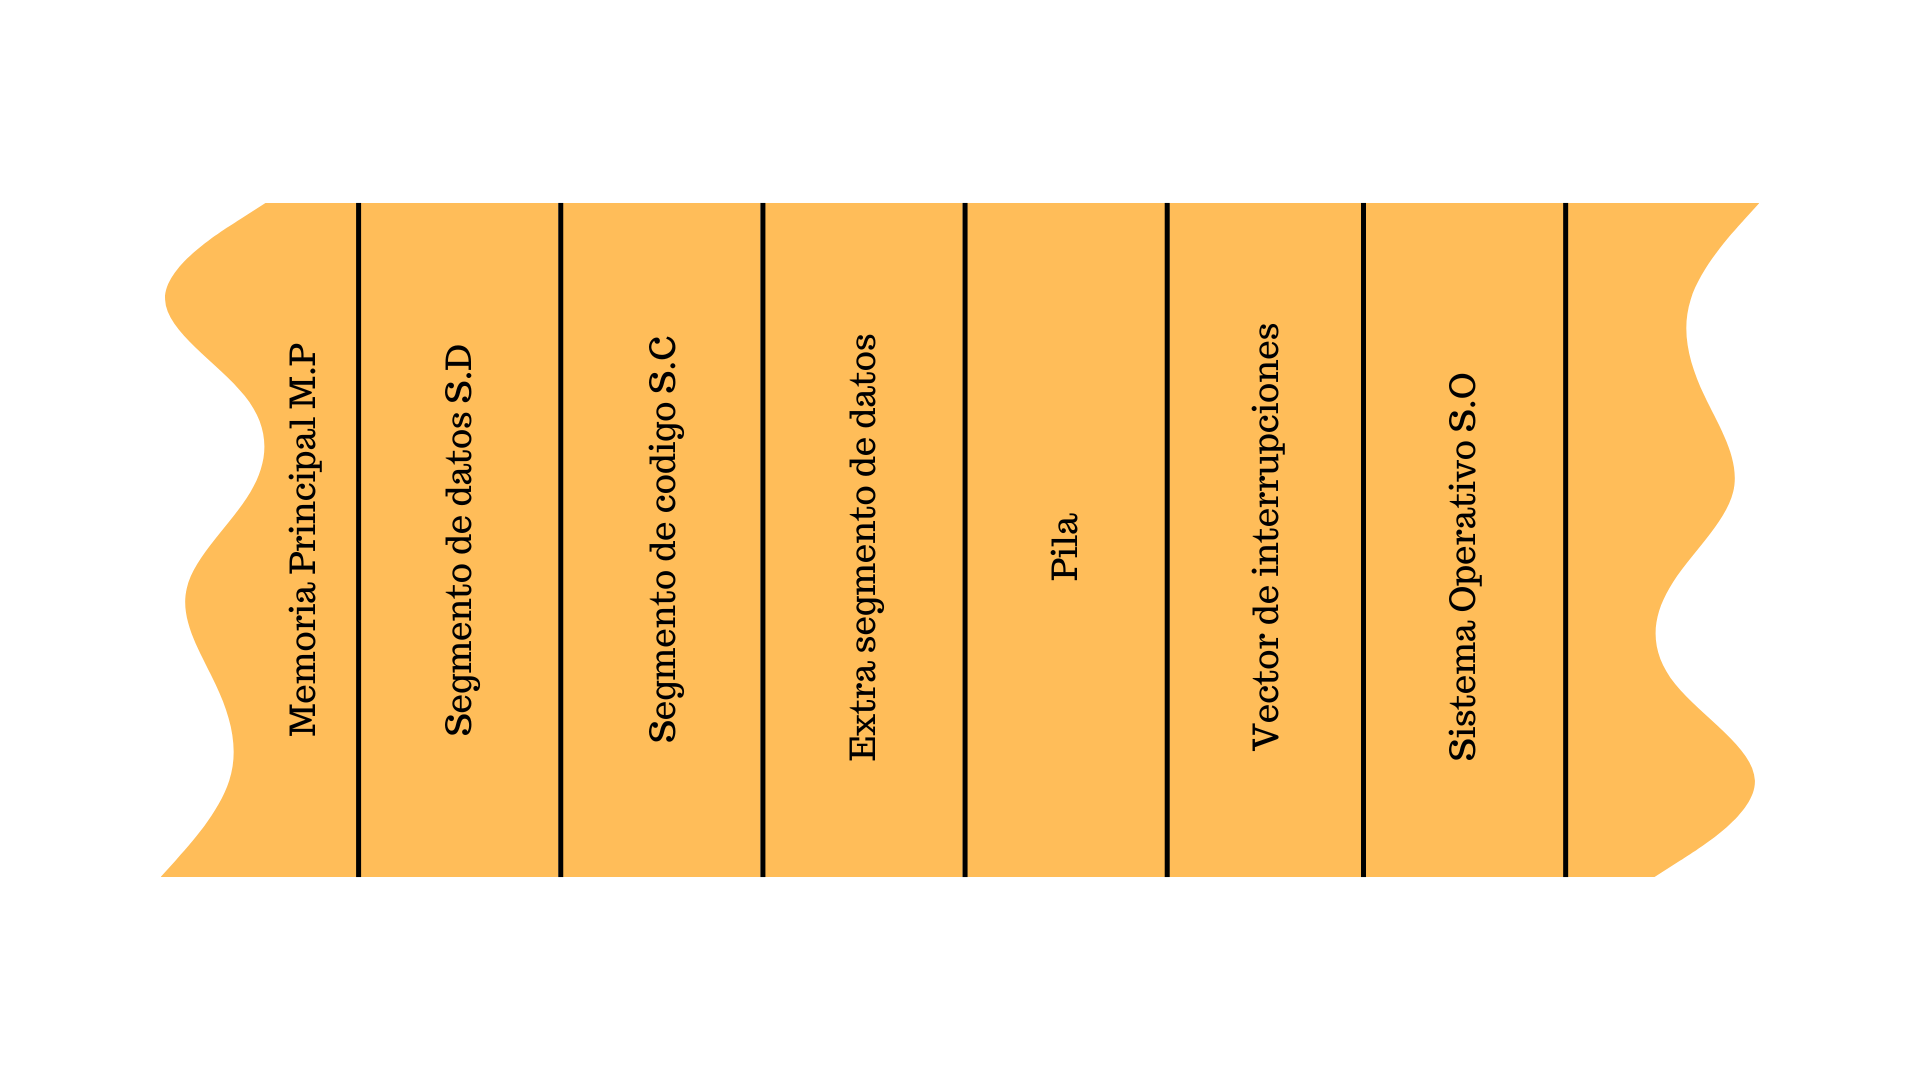
\includegraphics[height=5cm]{img/ram.png}}
\end{figure}

\noindent La imagen anterior representa a un modulo RAM, la cual en \hl{termino estricto} es homogénea, pero viene subdividido en sectores:
\begin{itemize}
    \item \textbf{Segmento de datos (S.D):} Se encarga del almacenamiento de datos, su tamaño es proporcional al tamaño de la memoria RAM.
    \item \textbf{Segmento de código (S.C):} Encargado de almacenar el programa (instrucciones), que vienen del disco de almacenamiento (disco duro).
    \item \textbf{Extra segmento de datos:} Un espacio extra en caso de que el tamaño en la S.D no sea el suficiente.
    \item \textbf{Pila:} Determina el orden de ejecución de transferencias de control. Almacena direcciones de memoria de donde ir al terminar cada instrucción 
    (transferencia de control en ciclos anidados) y datos de los parámetros de la instrucción (parámetros de ejecución).
    \item \textbf{Vector de interrupciones:} Vector dado por circuitos dentro de la RAM. Este se encarga de almacenar todos los microprogramas que manejan los 
    dispositivos internos de la computadora. En el vector de interrupciones se manejan todos los periféricos. Trabaja en conjunto con el \textbf{Runtime} 
    para saber que esta usando.
    \item \textbf{Sistema operativo S.O:} Es el encargado de manejar los recursos de la computadora.
\end{itemize}
\noindent Las variables pueden ser dinámicas o estáticas. Se tiende a usar dinámicas en la RAM para ahorrar espacio economizar recursos. Todos los datos se trabajan en 
SD y ExtraSD se pueden pedir estáticos o dinámicas(punteros). Los punteros pueden apuntar a una celda establecida o darle una celda propia con maloc.

\subsubsection{ROM (No volatil)}
\noindent La memoria ROM es una memoria de solo lectura, es decir, no se puede escribir en ella. Se utiliza para almacenar el programa de arranque de la computadora,

\subsubsection{Memoria caché}
\noindent La memoria caché es una memoria de acceso rápido que se encuentra entre la CPU y la memoria principal. Su función es almacenar los datos que se utilizan con mayor frecuencia,
\begin{itemize}
    \item \textbf{Ubicación:} Parte de la tarjeta madre y del procesador.
    \item \textbf{Uso:} Acceso rápido a la información por el procesador.
\end{itemize}

\subsection{Tarjetas de expansion interna}
\noindent Las tarjetas de expansión están diseñadas para actividades específicas como controlar la salida de video, gráficos y comunicaciones. Las principales tarjetas de expansión son:
\begin{itemize}
    \item \textbf{Tarjetas de video:} Controlan la salida de video.
    \item \textbf{Tarjetas de entrada y salida de datos:} Controlan la entrada y salida de datos.
    \item \textbf{Tarjetas de comunicaciones:} Controlan la comunicación entre la computadora y otros dispositivos.
\end{itemize}
\textbf{Tarjetas Controladoras de Comunicaciones} \\
Estas tarjetas permiten la conexión de una computadora con otras formando una red informática.\\
Tipos de redes y tarjetas:
\begin{itemize}
    \item Red de area local: Tarjeta de red \textbf{LAN} (NIC: Network Interface Card).
    \item Red de area extensa: Tarjeta de red \textbf{WAN}. Modem.
\end{itemize}

\subsection{Fuentes de alimentación}
\noindent Las fuentes de alimentación proporcionan la energía eléctrica que necesita la computadora para funcionar. Esa energía se estabiliza para impedir que la computadora se vea afectada por oscilaciones bruscas en el suministro de las compañías eléctricas.

\subsubsection{Valores de Voltaje} 
\noindent Típicamente se representan los 2 valores discretos de voltaje utilizados con las letras L y H, donde L es \textbf{LOW} y H es \textbf{HIGH}. 
\begin{table*} [H]
    \centering
    \colorbox{yellow!20}{%
        \begin{tabular}{|c|c|c|}
            \hline
            & \textbf{Alto/HIGH} & \textbf{Bajo/LOW}\\
            \hline
            Rangos de valores voltaje salida & [4 , 5.5] & [-0.5 , 1]\\
            \hline
        \end{tabular}
    }
    \label{tab:Voltajes}
    \caption*{\textbf{\textit{*Entra en el certamen según el profesor.}}}
\end{table*}

\noindent El procesador ejecuta el programa almacenado en el segmento de código, el cual se encuentra en la RAM utilizando los registros.

\subsection{Reloj}
\noindent El reloj de una computadora desempeña \textbf{dos funciones principales}. En primer lugar, \textbf{sincroniza diversas operaciones} que se realizan en diferentes componentes del sistema. 
En segundo lugar, sirve para \textbf{mostrar la hora actual}. La función principal es la primera, ya que ayuda a obtener el tiempo de ejecución (runtime) de las operaciones. \\\\
\textbf{Reloj del sistema:} Un pulso electrónico se utiliza para sincronizar el procesamiento en orden de nanosegundos, lo que permite medir el tiempo de ejecución (runtime) en MHz. 
Un megahercio (1 MHz) equivale a un millón de ciclos por segundo. 

\begin{tcolorbox}[colback=orange!10!white,colframe=orange!75!black,title=Observaciones]
    \begin{itemize}
        \item La frecuencia se refiere a cuantos instantes de atención a eventos/instrucciones se pueden realizar en un segundo.
        \item ROM es lo que sirve para arrancar y contiene el set-up.
        \item El lenguaje ensamblador le saca la máxima velocidad a la maquina.
        \item A lo que se refieren cuando dicen la maquina es de 2.4GHz es a la velocidad de su reloj, la cual es de 2.4 mil millones de ciclos por segundo.
    \end{itemize}
\end{tcolorbox}
\newpage

\section{Lenguaje Maquina}
\noindent Los códigos hexadecimales pueden representar instrucciones, registros de la CPU, direcciones de memoria o datos.
\begin{tcolorbox}[colback=blue!10!white,colframe=blue!75!black,title=Ejemplo]
    \begin{table}[H]
        \centering
            \begin{tabular}{|c|c|c|}
            \hline
            Código & Operación & Descripción \\
            \hline
            A0 & 2F & Acceder a la celda de memoria 2F \\
            3E & 01 & Copiar el registro 1 de la ALU \\
            A0 & 30 & Acceder a la celda de memoria 30 \\
            3E & 02 & Copiar en el registro 2 de la ALU \\
            1D & - & Sumar \\
            B3 & 31 & Guardar el resultado de la celda de memoria 31 \\
            \hline
            \end{tabular}
    \end{table}
\end{tcolorbox}
\subsection{Lenguaje Ensamblador}
\noindent El lenguaje ensamblador es un lenguaje de programación de bajo nivel que se utiliza para escribir programas que se ejecutan directamente en la CPU.
Se utilizan codificación nemotécnica para facilitar la programación y tener una mayor legibilidad.\\\\
\begin{minipage}[c]{0.5\textwidth}
\begin{table}[H]
    \centering
    \begin{tabular}{|c|c|}
    \hline
    READ & 2F \\
    REG & 01 \\
    READ & 30 \\
    REG & 02 \\
    ADD & - \\
    WRITE & 31 \\
    \hline
    \end{tabular}
\end{table}
\end{minipage}
\begin{minipage}[c]{0.5\textwidth}
\centering
\begin{tabular}{c}
    Código fuente (lenguaje ensamblador)\\
    $\downarrow$\\
    Programa ensamblador\\
    $\downarrow$\\
    Código máquina (lenguaje máquina)\\
\end{tabular}
\end{minipage}

\vspace{1cm} % Aumenta la separación vertical aquí

\noindent Este tipo de lenguaje se considera un \textbf{lenguaje de nivel medio}.\\\\

\subsection{Lenguajes de alto nivel}
\noindent Algunos lenguajes de alto nivel son: \\\\
\begin{minipage}{0.33\textwidth}
\begin{itemize}
    \item \textbf{Ada}
    \item \textbf{ALGOL}
    \item \textbf{BASIC}
    \item \textbf{C}
    \item \textbf{C++}
\end{itemize}
\end{minipage}
\begin{minipage}{0.33\textwidth}
\begin{itemize}
    \item \textbf{C\#}
    \item \textbf{COBOL}
    \item \textbf{Fortran}
    \item \textbf{Java}
    \item \textbf{Pascal}
\end{itemize}
\end{minipage}
\begin{minipage}{0.33\textwidth}
\begin{itemize}
    \item \textbf{Python}
    \item \textbf{Ruby}
    \item \textbf{Modula}
    \item \textbf{Simula}
\end{itemize}
\end{minipage}
\newpage

\section{Algebra de Boole}
\noindent George Boole introdujo el álgebra de Boole en 1854. Este sistema matemático se basa en la lógica y la teoría de conjuntos, y utiliza variables binarias (0 y 1) junto con compuertas lógicas para representar y manipular proposiciones lógicas. El álgebra de Boole es fundamental en la teoría de circuitos digitales y la informática.
\subsection{Compuertas lógicas}
\noindent Las compuertas lógicas son dispositivos electrónicos que realizan operaciones lógicas sobre una o más entradas binarias y generan una salida binaria. Las compuertas lógicas básicas son: \\\\
\begin{minipage}[t]{0.5\textwidth}
    \begin{center}
    \begin{itemize}
        \item \textbf{AND} 
        \item \textbf{OR} 
        \item \textbf{NOT}
        \item \textbf{NAND}
    \end{itemize}
    \end{center}
\end{minipage}%
\begin{minipage}[t]{0.5\textwidth}
    \begin{center}
    \begin{itemize}
        \item \textbf{NOR}
        \item \textbf{XOR}
        \item \textbf{XNOR}
    \end{itemize}
    \end{center}
\end{minipage}
\subsection{Compuertas lógicas básicas}
\subsubsection{Compuerta AND}
\noindent La compuerta AND produce una salida de 1 solo si todas sus entradas son 1. La tabla de verdad de una compuerta AND es: \\\\
\noindent % Asegura que las minipages comiencen en el borde izquierdo de la página % Asegura que las minipages comiencen en el borde izquierdo de la página
\begin{minipage}[c]{0.5\textwidth}
    \centering
    \begin{tabular}{|c|c|c|}
    \hline
    A & B & A AND B = A $\cdot$ B = Z\\
    \hline
    0 & 0 & 0 \\
    0 & 1 & 0 \\
    1 & 0 & 0 \\
    1 & 1 & 1 \\
    \hline
    \end{tabular}
\end{minipage}%
\begin{minipage}[c]{0.5\textwidth}
    \centering
    \begin{circuitikz}[transform shape, scale=1.5]
        % Ajusta la posición vertical aquí si es necesario
        \draw (0,0.75) node[and port] (myand1) {};
    \end{circuitikz}
\end{minipage}

\begin{tcolorbox}[colback=orange!10!white,colframe=orange!75!black,title=Observación]
    \textit{\textbf{Recordar que en un circuito representativo de AND en serie el voltaje total es la suma de los voltajes de las compuertas.-}}
\end{tcolorbox}

\subsubsection{Compuerta OR}
\noindent La compuerta OR produce una salida de 1 si al menos una de sus entradas es 1. La tabla de verdad de una compuerta OR es: \\\\
\noindent % Asegura que las minipages comiencen en el borde izquierdo de la página
\begin{minipage}[c]{0.5\textwidth}
    \centering
    \begin{table}[H]
        \centering
        \begin{tabular}{|c|c|c|}
        \hline
        A & B & A OR B = A + B = Z\\
        \hline
        0 & 0 & 0 \\
        0 & 1 & 1 \\
        1 & 0 & 1 \\
        1 & 1 & 1 \\
        \hline
        \end{tabular}
    \end{table}
\end{minipage}%
\begin{minipage}[c]{0.5\textwidth}
    \centering
    \begin{circuitikz}[transform shape, scale=1.5]
        % Ajusta la posición vertical aquí si es necesario
        \draw (0,0.75) node[or port] (myand1) {};
    \end{circuitikz}
\end{minipage}

\newpage


\subsubsection{Compuerta NOT}
\noindent La compuerta NOT produce una salida de 1 si su entrada es 0 y viceversa. La tabla de verdad de una compuerta NOT es:\\\\
\noindent % Asegura que las minipages comiencen en el borde izquierdo de la página
\begin{minipage}[c]{0.5\textwidth}
    \centering
    \begin{table}[H]
        \centering
        \begin{tabular}{|c|c|}
        \hline
        A & NOT A = $\overline{A}$ = Z\\
        \hline
        0 & 1 \\
        1 & 0 \\
        \hline
        \end{tabular}
    \end{table}
\end{minipage}%
\begin{minipage}[c]{0.5\textwidth}
    \centering
    \begin{circuitikz}[transform shape, scale=1.5]
        % Ajusta la posición vertical aquí si es necesario
        \draw (0,0.75) node[not port] (myand1) {};
    \end{circuitikz}
\end{minipage}

\subsection{Leyes del Algebra de Boole}
\textbf{Identidades Básicas} \\
\noindent % Asegura que las minipages comiencen en el borde izquierdo de la página
\begin{minipage}[t]{0.5\textwidth}
    \begin{enumerate}
        \item $X + 0 = X$
        \item $X + 1 = 1$
        \item $X + X = X$
        \item $X + \overline{X} = 1$
        \item $\overline{\overline{X}} = X$
    \end{enumerate}
\end{minipage}%
\begin{minipage}[t]{0.5\textwidth}
    \begin{enumerate}
        \setcounter{enumi}{5} % Continúa la numeración desde 6
        \item $X \cdot 0 = 0$
        \item $X \cdot 1 = X$
        \item $X \cdot X = X$
        \item $X \cdot \overline{X} = 0$
    \end{enumerate}
\end{minipage}
\vspace{0.5cm}

\noindent % Asegura que las minipages comiencen en el borde izquierdo de la página
\begin{minipage}[t]{0.375\textwidth}
    \begin{enumerate}
        \item $X + Y = Y + X$
        \item $X + (Y + Z) = (X + Y) + Z$
        \item $X(Y + Z) = XY + XZ$
        \item $\overline{X + Y} = \overline{X} \cdot \overline{Y}$
    \end{enumerate}
\end{minipage}%
\begin{minipage}[t]{0.375\textwidth}
    \begin{enumerate}
        \setcounter{enumi}{4} % Continúa la numeración desde 5
        \item $XY = YX$
        \item $X(YZ) = (XY)Z$
        \item $X + YZ = (X + Y)(X + Z)$
        \item $\overline{X \cdot Z} = \overline{X} + \overline{Z}$
    \end{enumerate}
\end{minipage}%
\begin{minipage}[t]{0.25\textwidth}
    \begin{enumerate}[label={}]
        \item Conmutativa
        \item Asociativa
        \item Distributiva
        \item De Morgan
    \end{enumerate}
\end{minipage}

\subsection{Compuertas lógicas avanzadas}
\subsubsection{Compuerta NAND}
\noindent La compuerta NAND produce una salida de 0 si todas sus entradas son 1. La tabla de verdad de una compuerta NAND es: \\\\  
\noindent % Asegura que las minipages comiencen en el borde izquierdo de la página
\begin{minipage}[c]{0.5\textwidth}
    \centering
    \begin{table}[H]
        \centering
        \begin{tabular}{|c|c|c|}
        \hline
        A & B & A NAND B = $\overline{A \cdot B}$ = Z\\
        \hline
        0 & 0 & 1 \\
        0 & 1 & 1 \\
        1 & 0 & 1 \\
        1 & 1 & 0 \\
        \hline
        \end{tabular}
    \end{table}
\end{minipage}%
\begin{minipage}[c]{0.5\textwidth}
    \centering
    \begin{circuitikz}[transform shape, scale=1.5]
        % Ajusta la posición vertical aquí si es necesario
        \draw (0,0.75) node[nand port] (myand1) {};
    \end{circuitikz}
\end{minipage}
\subsubsection{Compuerta NOR}
\noindent La compuerta NOR produce una salida de 1 si todas sus entradas son 0. La tabla de verdad de una compuerta NOR es: \\\\  
\noindent % Asegura que las minipages comiencen en el borde izquierdo de la página
\begin{minipage}[c]{0.5\textwidth}
    \centering
    \begin{table}[H]
        \centering
        \begin{tabular}{|c|c|c|}
        \hline
        A & B & A NOR B = $\overline{A + B}$ = Z\\
        \hline
        0 & 0 & 1 \\
        0 & 1 & 0 \\
        1 & 0 & 0 \\
        1 & 1 & 0 \\
        \hline
        \end{tabular}
    \end{table}
\end{minipage}%
\begin{minipage}[c]{0.5\textwidth}
    \centering
    \begin{circuitikz}[transform shape, scale=1.5]
        % Ajusta la posición vertical aquí si es necesario
        \draw (0,0.75) node[nor port] (myand1) {};
    \end{circuitikz}
\end{minipage}

\subsubsection{Compuerta XOR}
\noindent La compuerta XOR produce una salida de 1 si sus entradas son diferentes. La tabla de verdad de una compuerta XOR es: \\\\  
\noindent % Asegura que las minipages comiencen en el borde izquierdo de la página
\begin{minipage}[c]{0.5\textwidth}
    \centering
    \begin{table}[H]
        \centering
        \begin{tabular}{|c|c|c|}
        \hline
        A & B & A XOR B = Z\\
        \hline
        0 & 0 & 0 \\
        0 & 1 & 1 \\
        1 & 0 & 1 \\
        1 & 1 & 0 \\
        \hline
        \end{tabular}
    \end{table}
\end{minipage}
\begin{minipage}[c]{0.5\textwidth}
    \centering
    \begin{circuitikz}[transform shape, scale=1.5]
        % Ajusta la posición vertical aquí si es necesario
        \draw (0,0.75) node[xor port] (myand1) {};
    \end{circuitikz}
\end{minipage}

\section{Simplificación de funciones lógicas (Mapas de Karnaugh)} 
\noindent Los mapas de Karnaugh son una herramienta gráfica que se utiliza para simplificar funciones lógicas. Los mapas de Karnaugh son especialmente útiles para simplificar funciones lógicas con hasta 4 variables.\\\\
\textbf{Pasos para simplificar funciones lógicas con mapas de Karnaugh:}
\begin{enumerate}
    \item \textbf{Identificar las variables:} Identificar las variables de la función lógica.
    \item \textbf{Crear el mapa de Karnaugh:} Crear un mapa de Karnaugh con las variables identificadas.
    \item \textbf{Completar el mapa de Karnaugh:} Completar el mapa de Karnaugh con los valores de la función lógica.
    \item \textbf{Simplificar la función lógica:} Utilizar el mapa de Karnaugh para simplificar la función lógica.
\end{enumerate}
\begin{tcolorbox}[colback=blue!10!white,colframe=blue!75!black,title=Ejemplo]
    Para la tabla de verdad de la función lógica $F(A,B,C)$:
    \begin{table}[H]
        \centering
        \begin{tabular}{|c|c|c|c|}
        \hline
        A & B & C & F\\
        \hline
        \rowcolor{purple!30} 0 & 0 & 0 & \cellcolor{purple}1\\
        \rowcolor{purple!30} 0 & 0 & 1 & \cellcolor{purple}1\\
        0 & 1 & 0 & 0\\
        \rowcolor{purple!30} 0 & 1 & 1 & \cellcolor{purple}1\\
        1 & 0 & 0 & 0\\
        \rowcolor{purple!30} 1 & 0 & 1 & \cellcolor{purple}1\\
        1 & 1 & 0 & 0\\
        1 & 1 & 1 & 0\\
        \hline
        \end{tabular}
    \end{table}
Por lo que a simple vista podemos concluir la siguiente función lógica:
\begin{itemize}
    \item $F = \colorbox{blue!30}{$\overline{ABC}$} + \colorbox{yellow}{$\overline{AB}C$} +  \colorbox{green}{$\overline{A}BC$} + \colorbox{red}{$A\overline{B}C$}$
\end{itemize}
Por lo tanto la construcción de un mapa de Karnaugh para la función lógica $F(A,B,C)$ es:
\begin{center}
    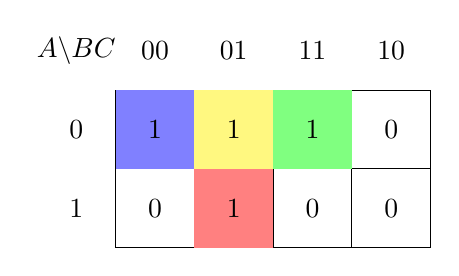
\begin{tikzpicture}
        % Dibuja las celdas del mapa de Karnaugh
        \draw (0,0) grid (4,2);
        
        % Etiquetas de las columnas (combinaciones de B y C)
        \node at (0.5, 2.5) {00};
        \node at (1.5, 2.5) {01};
        \node at (2.5, 2.5) {11};
        \node at (3.5, 2.5) {10};
        
        % Etiquetas de las filas (valor de A)
        \node at (-0.5, 1.5) {0};
        \node at (-0.5, 0.5) {1};
        
        % Añadir etiqueta "A\BC" en el cruce entre filas y columnas
        \node at (-0.5, 2.5) {$A\backslash BC$};
        
        % Rellenar las celdas según la función lógica F
        \fill[blue!50] (0,1) rectangle (1,2); % ABC'
        \fill[yellow!50] (1,1) rectangle (2,2); % AB'C
        \fill[green!50] (2,1) rectangle (3,2); % A'BC
        \fill[red!50] (1,0) rectangle (2,1); % A'B'C
        
        % Añadir etiquetas de minterminos
        \node at (0.5, 1.5) {1};
        \node at (1.5, 1.5) {1};
        \node at (2.5, 1.5) {1};
        \node at (1.5, 0.5) {1};
        
        % Añadir etiquetas de 0 en las celdas restantes
        \node at (3.5, 1.5) {0}; % A'BC'
        \node at (0.5, 0.5) {0}; % A'B'C'
        \node at (2.5, 0.5) {0}; % A'BC'
        \node at (3.5, 0.5) {0}; % A'BC'
    \end{tikzpicture}
\end{center}
Lo cual al reducir los grupos de 1's obtenemos la función lógica simplificada tenemos que para:
\begin{itemize}
    \item El grupo azul-amarillo representa la combinación $\overline{A}B$
    \item El grupo rojo-amarillo representa la combinación $B\overline{C}$
    \item El grupo verde-amarillo representa la combinación $\overline{A}C$
\end{itemize} 
Por lo que la función lógica simplificada es:
\begin{center}
    \textbf{$F = \overline{A}B + B\overline{C} + \overline{A}C$}       
\end{center}
\end{tcolorbox}
\newpage

\section{Sistemas numéricos digitales}
\subsection{Abstracción digital}
\begin{itemize}
    \item La mayoría de las variables son \textbf{continuas}.
    \begin{itemize}
        \item Voltaje de un cable.
        \item Frecuencia de un oscilador.
        \item Posición de un objeto.
    \end{itemize}
    \item La abstracción digital considera un \textbf{conjunto discreto} de valores (0,1,2,...).
\end{itemize}

\subsection{Disciplina digital}
\begin{itemize}
    \item Dos valores discretos:
    \begin{itemize}
        \item 1's y 0's.
        \item 1 $\rightarrow$ Verdadero/True, Alto/High.   
        \item 0 $\rightarrow$ Falso/False, Bajo/Low. 
    \end{itemize}
    \item \textbf{1 y 0}: Niveles de voltaje, engranajes giratorios, niveles de fluidos, etc.
    \item Los circuitos de digitales usan niveles de \textbf{voltaje} para representar 1's y 0's.
    \item \textbf{Bit:} Dígito binario, unidad más pequeña de información.
\end{itemize}

\subsection{Sistemas de numeración}
\noindent El sistema numérico decimal es el más común, pero existen otros sistemas de numeración que se utilizan en la informática y la electrónica digital. Los sistemas de numeración más comunes son:
\begin{itemize}
    \item \textbf{Binario:} Base 2.
    \item \textbf{Octal:} Base 8.
    \item \textbf{Hexadecimal:} Base 16.
    \item \textbf{Decimal:} Base 10.
\end{itemize}

\subsubsection{Rangos y valores}
\noindent A través del sistema binario y decimal existen diferentes rangos de valores que se pueden representar, los cuales podemos calcular de la siguiente manera:
\begin{itemize}
    \item Números decimales de $n$ dígitos:
    \begin{itemize}
        \item Valores distintos con $n$ dígitos: $10^n$
        \item Rango de valores con $n$ dígitos: $0$ a $10^n - 1$ 
    \end{itemize}
    \item Números binarios de $n$ bits:
    \begin{itemize}
        \item Valores distintos con $n$ bits: $2^n$
        \item Rango de valores con $n$ bits: $0$ a $2^n - 1$
    \end{itemize}   
\end{itemize}

\subsubsection{Conversión de sistemas de numeración}
\textbf{Conversión binaria a decimal:}
\begin{itemize}
    \item \textbf{Ejemplo:} Convertir el número binario 1011 a decimal.
    \begin{itemize}
        \item $1 \cdot 2^3 + 0 \cdot 2^2 + 1 \cdot 2^1 + 1 \cdot 2^0 = 8 + 0 + 2 + 1 = 11$
    \end{itemize}
\end{itemize}
\textbf{Conversión decimal a binario:}
\begin{itemize}
    \item \textbf{Ejemplo:} Convertir el número decimal 13 a binario.
        \begin{itemize}
            \item $13 \div 2 = 6$ con residuo $1$
            \item $6 \div 2 = 3$ con residuo $0$
            \item $3 \div 2 = 1$ con residuo $1$
            \item $1 \div 2 = 0$ con residuo $1$
        \end{itemize}
    Por lo tanto, el número decimal 13 en binario es $1101$.
\end{itemize}
\textbf{Conversión binaria a hexadecimal:}
\begin{itemize}
    \item \textbf{Ejemplo:} Convertir el número binario 101101 a hexadecimal.
    \begin{itemize}
        \item $101101 = 1 \cdot 2^5 + 0 \cdot 2^4 + 1 \cdot 2^3 + 1 \cdot 2^2 + 0 \cdot 2^1 + 1 \cdot 2^0 = 32 + 0 + 8 + 4 + 0 + 1 = 45$
        \item $45 = 2 \cdot 16^1 + 13 \cdot 16^0 = 2D$
    \end{itemize}
\end{itemize}
\textbf{Conversión hexadecimal a binario:}
\begin{itemize}
    \item \textbf{Ejemplo:} Convertir el número hexadecimal 2D a binario.
    \begin{itemize}
        \item $2D = 2 \cdot 16^1 + 13 \cdot 16^0 = 45$
        \item $45 = 32 + 8 + 4 + 1 = 101101$
    \end{itemize}
\end{itemize}
\textbf{Conversión decimal a hexadecimal:}
\begin{itemize}
    \item \textbf{Ejemplo:} Convertir el número decimal 45 a hexadecimal.
    \begin{itemize}
        \item $45 = 2 \cdot 16^1 + 13 \cdot 16^0 = 2D$
    \end{itemize}
\end{itemize}
\textbf{Conversión hexadecimal a decimal:}
\begin{itemize}
    \item \textbf{Ejemplo:} Convertir el número hexadecimal 2D a decimal.
    \begin{itemize}
        \item $2D = 2 \cdot 16^1 + 13 \cdot 16^0 = 45$
    \end{itemize}
\end{itemize}
\textbf{Conversión octal a decimal:}
\begin{itemize}
    \item \textbf{Ejemplo:} Convertir el número octal 45 a decimal.
    \begin{itemize}
        \item $45 = 4 \cdot 8^1 + 5 \cdot 8^0 = 37$
    \end{itemize}
\end{itemize}
\textbf{Conversión decimal a octal:}
\begin{itemize}
    \item \textbf{Ejemplo:} Convertir el número decimal 182 a octal.
        \begin{itemize}
            \item $182 \div 8 = 22$ con residuo $6$
            \item $22 \div 8 = 2$ con residuo $6$
            \item $2 \div 8 = 0$ con residuo $2$
        \end{itemize}
    Por lo tanto, el número decimal 182 en octal es $266$.
\end{itemize}

\subsection{Bits, Bytes, Nibbles,...}
\noindent Los \textbf{bits} son la unidad mas pequeña de información, los cuales se agrupan, dando a conocer un rango de importancia dependiendo de la ubicación de los bits. Por ejemplo:
\begin{center}
    \textit{Most significant bit}[MSB]$\rightarrow$\colorbox{blue!30}{1}10101\colorbox{blue!30}{0}$\leftarrow$\textit{Least significant bit}[LSB]
\end{center}

\noindent A la agrupación de estos bits se les conoce como \textbf{Bytes}, los cuales son de 8 bits. A su vez, los bytes se pueden agrupar en \textbf{Nibbles}, los cuales son de 4 bits.Por lo tanto, un byte es igual a 2 nibbles.
\begin{center}
    \begin{tabular}{|c|c|c|c|c|c|c|c|c|c|}
    \hline
    Byte & 1 & 0 & 1 & 0 & 1 & 0 & 1 & 0 \\
    \hline
    Nibble 1 & 1 & 0 & 1 & 0 & - & - & - & - \\
    Nibble 2 & - & - & - & - & 1 & 0 & 1 & 0 \\
    \hline
    \end{tabular}
\end{center}


\end{document}
 